\subsection{Introduction}
The Task for the second phase was to calculate the building's energy demand using Java with the citygml4j library and the 3D city model. Necessary for that are the building’s volume and the attribution of walls as outer- or inner-/shared- wall surfaces which already was calculated by group one in phase one.\\
The most important information for this task are content of the so called IWU Report which is a report created by the IGG (Institute for Geodesy and Geoinformation Science) based on calculation methods of the "Institut Wohnen und Umwelt GmbH" [eng. Institute living and environment GmbH]. The IWU Report can be interpreted as a manual for the calculation of the building energy demand using the semantic citymodel of Berlin.\\
The document is structured into three parts: The determination of the input-values which are temperature, geometries and energy reference building-parameter, the calculation of the building's energy demand for space-heating using an accounting system and the calculation of the building's energy demand for warm-water.

\subsection{Input values}
For the calculation of energy flow of buildings, the surrounding climate is of an big importance. To take this into account some formulas contain a variable called "Gradstunden" which is representing the climate in a numerical value. For its calculation the summed up days per year have to be multiplied with the difference of the heated temperature inside and the actual temperature outside. To neglect the summer season in which buildings do not need any external heating energy, only the days with a switched on heater were considered.\\
The energy reference area is relevant for all calculations dealing with the building size. And due to the fact, that a precise indoor-model of the city is not available, the estimation of this value can be done with the formula (\ref{eq:energyReferenceArea}). Important to know is that only heated storeys without roof and cellar are taken into account.
\begin{equation}
	A_{EB} = 0.75 \times n_{G} x A_{FB} [m^2]
	\label{eq:energyReferenceArea}
\end{equation}
\begin{description}
	\item[$n_{G}$:] number of storeys
	\item[$A_{FB}$:] building footprint
\end{description}
Necessary for air-volume calculations inside, either the precise storey height have to known, or the average storey height which is depending on type and age of the building. Figure \ref{fig:storeyHeight} shows some average values of storey height depending on the building's age. Furthermore we took for our calculations additional 0.3m per storey in order to achieve (more or less) the same number of storeys as in real world. This number was found be supervising some samples of buildings which are part in our database-subset.
\begin{figure}[h]
	\centering
 	 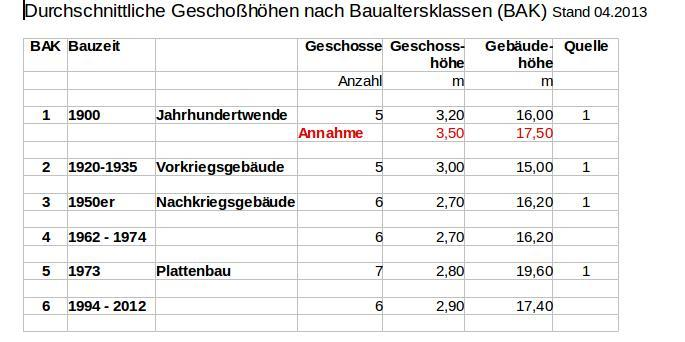
\includegraphics[scale=0.5]{phase2/group1/storey_height.jpg} 
	\caption{Average storey height depending on building's age. Provided by Michael Prytula.}
	 \label{fig:storeyHeight}
\end{figure}
The air-volume then can be calculated with the formula (\ref{eq:airVolume}) which is the energy reference area multiplied with the assumed mean (lighted) storey height.
\begin{equation}
	V_L = A_{EB} \times 2.5
	\label{eq:airVolume}
\end{equation}
Since some energy flows through building parts, its physical behaviour has be taken into account when calculation the energy flow. For this issue the so called U-values (in the IWU-Report called "k-Werte") are needed. They are describing the amount of energy transmitting between different building parts as for example between building-roof and building-main-part. Due to the fact that energy will not flow between two parts having the same temperature, it is important to know which wall surfaces are shared with also heating neighboured buildings. Figure \ref{fig:uValues} shows possible directions of the energy transmission, and possible building parts differentiated by its mean temperature. The afterwards following figure \ref{fig:uValuesTable} shows average U-values for specific building-ages and building-parts.
\begin{figure}[h]
	\centering
 	 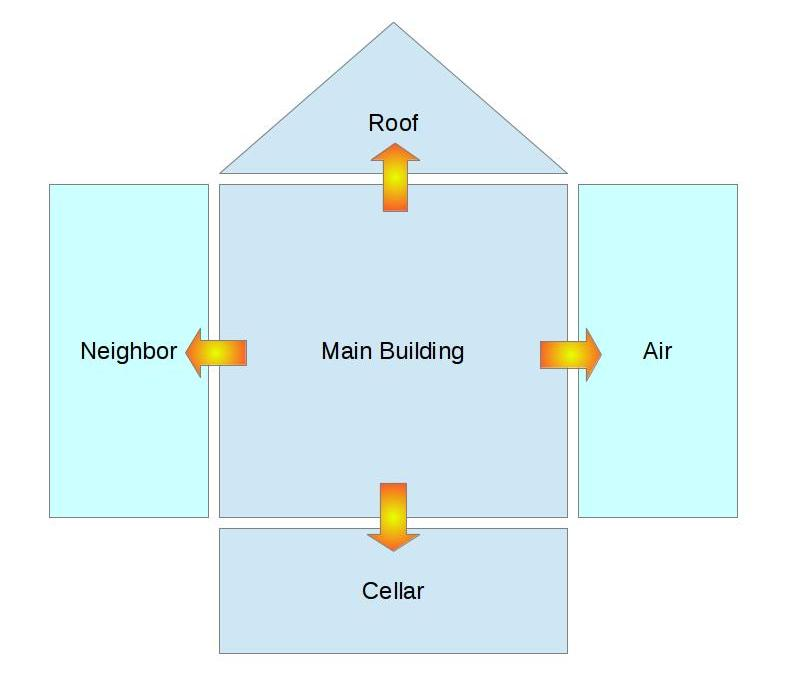
\includegraphics[scale=0.4]{phase2/group1/U-Values.jpg}
	\caption{Possible energy flow directions of a building.}
	\label{fig:uValues}
\end{figure}
\begin{figure}[h]
	\centering
 	 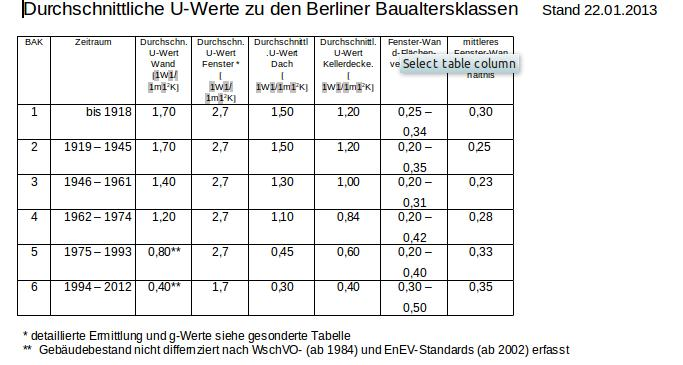
\includegraphics[scale=0.59]{phase2/group1/u-values_table.jpg}
	\caption{Average U-Values for specific building-ages and building-parts. Provided by Michael Prytula.}
	\label{fig:uValuesTable}
\end{figure}

\subsection{Demand of effective energy for heating}
The following formulas are describing the sequence of calculating the effective energy demand for heating. Later on following formulas are partially depending on the previous ones.\\
The calculation of the energy demand for heating can be easily done with using an accounting system as follows (\ref{eq:heatingDemand}):
\begin{equation}
Demand = Gain - Loss
\label{eq:heatingDemand}
\end{equation}
The Energy loss in [kWh/a] can be calculated as follows (\ref{eq:energyLoss}). 
\begin{equation}
Q_{V} = (Q_T + Q_L) \times f_{Abs}
\label{eq:energyLoss}
\end{equation}
\begin{description}
\item[$Q_{T}$:] transmission loss [kWh/a]
\item[$Q_L$: ]aeration loss [kWh/a]
\item[$f_{Abs}$:] reduction factor day-/night-setback
\end{description}
The values for the specific Day-nightsetback can be taken from a table with average values, depending on the building type (e.g. new-building).\\
The loss through transmission in [kWh/a] has to be taken from this formula (\ref{eq:lossTransmission}):
\begin{equation}
Q_T = (\sum f_i \times k_I \times A_i) \times \Theta 
\label{eq:lossTransmission}
\end{equation}
\begin{description}
\item[$f_i$:]reductionfactor [1.0 outer-walls; 0.5 inner-walls]
\item[$k_I$:] U-value [W/($m2$K)]
\item[$A_i$:] building's area [$m^2$]
\item[$\Theta$:] Gradstunden [kKh/a]
\end{description}
Summed up for every building part [i].\\
The loss through aeration in [kWh/a] can be calculated using the formula (\ref{eq:lossAeration}):
\begin{equation}
Q_L = 0.34 \times n \times V_L \times \Theta 
\label{eq:lossAeration}
\end{equation}
\begin{description}
\item[$n$:] frequency of aeration [1/h] (from table)
\item[$V_L$:] building's air volume [$m^3$]
\end{description}
For the energy gain following formulas have to be applied:\\
In general formula (\ref{eq:energyGain}) is describing the utilisation of the available free heat inside of the building:
\begin{equation}
Q_G = \eta_F \times Q_F 
\label{eq:energyGain}
\end{equation}
\begin{description}
\item[$\eta_F$:] utilisation
\item[$Q_F$:] free heat
\end{description}
The free heat is simply the solar irradiation plus the heat sources inside of the building (see formula (\ref{eq:freeHeat})).
\begin{equation}
Q_F = Q_S + Q_I 
\label{eq:freeHeat}
\end{equation}
\begin{description}
\item[$Q_S $:] solar irradiation
\item[$Q_I $:] heat sources inside
\end{description}
And following formula (\ref{eq:utilisation}) can be used for the utilisation:
\begin{equation}
\eta_F = 1 - 0.3 \times (\dfrac{Q_F}{Q_V}) 
\label{eq:utilisation}
\end{equation}
\begin{description}
\item[$Q_V $:] (remember:) energy-loss
\end{description}
As important income the solar energy gain can be calculated with the precise formula (\ref{eq:solarGain}) which needs precise knowledge about the window sizes.
\begin{equation}
Q_S = r \times g_{senkr} \times \sum G_i \times A_{F,i} 
\label{eq:solarGain}
\end{equation}
\begin{description}
\item[$G_i $:] global radiation per orientation (e.g. south)
\item[$A_{F,i} $:] window area per orientation [$m^2$]
\item[$g_{senkr} $:] energy transmission through glass-area (from Kurzverfahren Energieprofil)
\item[$r $:] reduction factor due to windows (standard value: 0.36)
\end{description}
Taking an factor for the window sizes per wall, also the following simplified formula (\ref{eq:simplySolarGain}) can be used for the calculations.
\begin{equation}
Q_S = r \times g_{senkr} \times 240 \times A_{window} 
\label{eq:simplySolarGain}
\end{equation}
\begin{description}
\item[$A_{window} $:] estimated overall window area [$m^2$]
\end{description}
Inside of buildings there are more heat sources than only the heater. For example electric devices like the light bulb are producing a lot of heat energy, which is also a factor for the calculations.\\
As a assumption, the next formula (\ref{eq:innerHeatSources}) is giving this factor a size.
\begin{equation}
Q_I = 0.024 \times q_i \times t_H \times A_{EB} 
\label{eq:innerHeatSources}
\end{equation}
\begin{description}
\item[$0.024 $:] factor for conversation ([W] $\rightarrow$ [kW]; [d] $\rightarrow$ [h]
\item[$q_i $:] specific power of inside heat sources [W/$m^2$]
\item[$t_H $:] heating period [d/a]
\item[$A_{EB} $:] energy reference area
\end{description}

\subsection{Demand of effective energy for warmwater}
The demand of warm water [kWh/a] can more easily be calculated. It is simply the demand per person multiplied with the number of persons living in the building. The formula (\ref{eq:warmWater}) shows how this can be calculated.
\begin{equation}
Q_W = \dfrac{Q_{W/P} \times A_{EB}}{A_{EB/P}}
\label{eq:warmWater}
\end{equation}
\begin{description}
\item[$Q_{W/P} $:] demand of warm water per year and person [kWh/(P a)] (standard: 600 kWh/(P a))\\
\item[$A_{EB/P} $:] living space per person [$m^2$/P] (standard: 35 $m^2$/P)\\
\end{description}
This formula calculates the number of persons living in the building by dividing the energy related area by the average space per person. When having a more precise estimation of inhabitants per building as group three was calculating, the formula can be changed into the formula (\ref{eq:simplyWarmWater}):
\begin{equation}
Q_W = Q_{W/P} \times N_P
\label{eq:simplyWarmWater}
\end{equation}
\begin{description}
\item[$N_P$:] number of persons\\
\end{description}

\subsection{Result}
As results of the calculations, the Java algorithm produces a .csv file containing information about each building which has an own identifier. All values are calculated in [kWh/a]. The table shows a subset of the result file, with three buildings and the interesting attributes described in this report.
\begin{table}[b]
\centering
\begin{tabular}{c  c  c  c  c  c}
building\_id & heating\_loss & heating\_gain & ... & ..demand\_heating & ..demand\_warmwater \\
\hline						
BLDG\_000300000026ed79 & 116670,763	& 15572,718 & ... & 101098,045 & 4805,405\\
BLDG\_000300000026f491 & 229314,037	& 32343,216 & ... & 196970,821 & 16289,207\\
BLDG\_000300000026f4a7 & 216882,225	& 31687,923 & ... & 185194,302 & 15044,102\\
...\\
\end{tabular}
\label{table:result IWU-Report}
\caption{Results of the IWU-report-calculation [kWh/a].} 
\end{table}

\subsection{Discussion}
The number of storeys is one central value of all calculation, because with a wrong estimated number of storeys the reference are can change rapidly. Figure \ref{fig:changeArea} shows how the reference area is changing with the wrong estimated number of storeys.
\begin{figure}[h]
	\centering
 	 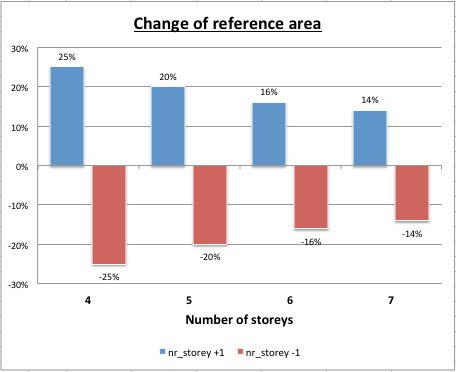
\includegraphics[scale=0.5]{phase2/group1/change_area.png} 
	\caption{Changing area with wrong estimated number of storeys.}
	 \label{fig:changeArea}
\end{figure}
And therewith also the calculated energy parameters which are depending on the reference area are changing.  Figure \ref{fig:changeParameter} shows how strong they are depending on a right estimated number of storeys.
\begin{figure}[h]
	\centering
 	 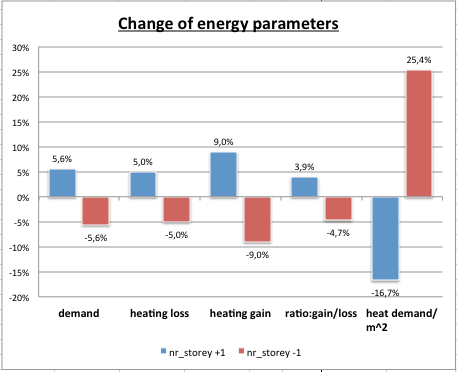
\includegraphics[scale=0.5]{phase2/group1/change_param.png} 
	\caption{Changing energy parameters with wrong estimated number of storeys.}
	 \label{fig:changeParameter}
\end{figure}

Following improvements could be helpful to obtain better results:\\
First as mentioned before we took additional 0.3m to obtain a better estimation, this is because in the calculations the average storey height was describing the inside storey height without ceiling thickness.\\
Maybe it would be useful to consider the building's usage for the estimation of the specific storey height.\\
In the IWU report 2.5m were assumed as the storey height for the air-volume, in our calculations we were using the previously calculated storey height.
